\subsection{Memory Affinity}
\label{sub:memory_affinity}

%% BRONIS: I moved hierarchical to the previous section
%% BRONIS: I think we can still say something on affinity a la Data Tsar

While the near-term goals include using memory location information to inform
task affinity, as discussed in Section~\ref{sub:new_tasking}, one of the
longer-term goals is to introduce more general memory affinity into OpenMP.  One
of the interfaces we've explored for this accomplishes it by associating data to
computation, then using the normal distribution of computation onto compute
resources appropriately locates, transforms or replicates data.  A prototype
version~\cite{ctsar-tpds,scogland:7Hpt64iV} has been produced that works for a
subset of the solution space.  More recent developments could allow code as presented
in Figure~\ref{fig:atsar-gemm} to partition a logical range across threads in a
\texttt{parallel} region, or target devices in a system, or an arbitrary nesting
thereof.

\begin{figure}
\begin{minted}{c}
int i, i_start=0, i_end=i_size, j, j_start=0, j_end=j_size;
float A[k_size][j_size], B[i_size][k_size];
float *C = (float*)malloc(sizeof(C[0])*i_size*j_size);
int   C_pitch = j_size;

#pragma omp parallel devices(socket)
 partition(adaptive: j_id=j_start; j_id<j_end; ++j_id)         \
 map(to: A[0:k_size][:,partition=j_id], B[0:i_size][0:k_size]) \
 map(tofrom: C[0:i_size,pitch=C_pitch][:,partition=j_id])
{ // Partitioned parallel region
#pragma omp target teams distribute parallel for  \
  devices(all) partition(dynamic)                 \
  map(to: A[:][:], B[:,partition=i][:])           \
  map(tofrom: C[:,partition=i][:])
  for (int i = i_start; i < i_end; ++i) { // Partitioned loop
    for (int j = j_start; j < j_end; ++j) {
      float sum = 0.0;
      for (int k = 0; k < k_size; ++k) {
        sum += A[k][j] * B[i][k];
      }
      C[i * C_pitch + j] = sum;
    }
  }
}
\end{minted}
\caption{A possible interface to partition memory for affinity.\label{fig:atsar-gemm}}
\end{figure}

The code in Figure~\ref{fig:atsar-gemm} would partition the GEMM loop into
two-dimensional tiles by columns across sockets and rows across devices
associated with a given socket.  Extensions like this require careful
consideration due to their potentially large number of changes, and high
complexity, but the optimizations permitted by providing this level of
information to the compiler can be significant.  Beyond providing affinity
information, these annotations are sufficient to allow for cross-device
coscheduling across non-shared-memory devices.  Figure~\ref{fig:atsar-perf}
shows performance results from a prototype implementation across five benchmark
kernels in terms of speedup over a baseline OpenMP static schedule using all
cores.  The annotations and scheduling improvements they allow for increase
performance even on CPU alone, and in all but one case gain yet more from
co-scheduling across CPU and GPU devices.


\begin{figure*}[t]
        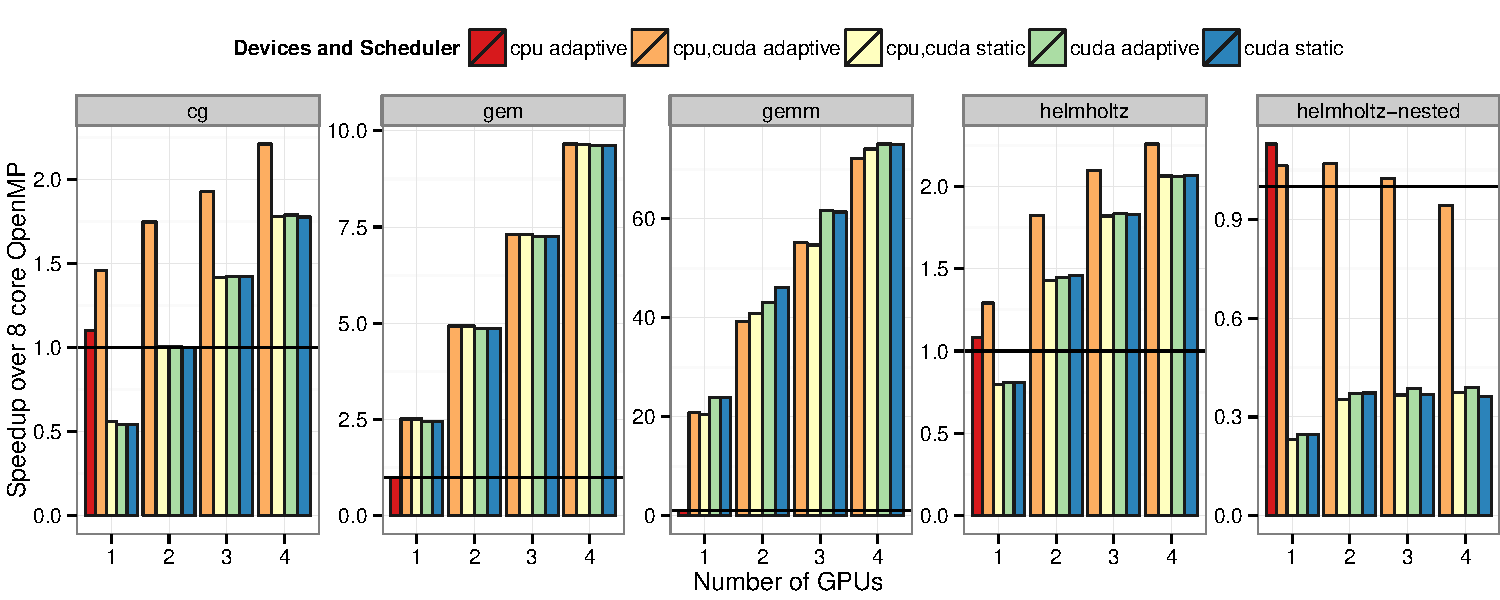
\includegraphics[width=\textwidth]{system-1-combined-part}
        \caption{Memory partitioning/affinity performance combined with
        cross-device coscheduling enabled by the same
      extensions.\label{fig:atsar-perf}}
\end{figure*}


